\subsection{\highlight{Multi-Dimensional Evaluation}}

We first report multi-dimensional evaluation results across all baselines.
Table \ref{table:evaluation_results} shows mean scores across eight evaluation criteria along with standard deviation values.
Figure~\ref{figure:evaluation_results} provides a visual comparison of the reasoning profiles across the evaluated methods.
While most methods achieve relatively high scores on structural dimensions such as coherence and decomposition, FP2MP demonstrates a more pronounced advantage on reflective dimensions, particularly framing, justification, metacognition, and uncertainty handling.
The figure also highlights that ReAct and Actor-Critic remain competitive on several structural and knowledge-related dimensions.


\begin{table}[h]
\centering
\small
\resizebox{\textwidth}{!}{
\begin{tabular}{lcccccll}
\hline
\textbf{Criterion} & \textbf{Single Agent}  
& \textbf{Chain-of-Thought} & \textbf{Actor-Critic} & \textbf{ReAct} 
& \textbf{Majority Voting} 
&\textbf{Debate}
&\textbf{FP2MP}\\
\hline
Coherence & 4.17 ± 0.38  
& 4.13 ± 0.34 & 4.44 ± 0.50 & \underline{4.53 ± 0.50} 
& 3.94 ± 0.61 
&4.17 ± 0.47  &4.39 ± 0.52\\
Decomposition & 4.14 ± 0.35  
& 4.09 ± 0.29 & 4.38 ± 0.49 & \underline{4.44 ± 0.50} 
& 3.89 ± 0.62 
&4.13 ± 0.43  &4.15 ± 0.47\\
Diversity & 3.32 ± 0.62  
& 2.81 ± 0.64 & 3.41 ± 0.56 & 3.36 ± 0.55 
& 3.04 ± 0.80 
&3.10 ± 0.62  & \underline{3.55 ± 0.54}\\
Framing & 4.19 ± 0.39  
& 4.05 ± 0.28 
& 4.44 ± 0.50 & 4.41 ± 0.49 
& 3.92 ± 0.64 
&4.15 ± 0.45  & \underline{4.58 ± 0.49}\\
Justification & 3.45 ± 0.50  
& 3.16 ± 0.36 
& 3.91 ± 0.35 & 3.77 ± 0.48 
& 3.09 ± 0.64 
&3.37 ± 0.55  & \underline{4.36 ± 0.56}\\
Knowledge Integration & 4.28 ± 0.45  
& 4.13 ± 0.40 
& 4.53 ± 0.50 & \underline{4.67 ± 0.47} 
& 3.97 ± 0.67 
&4.22 ± 0.50  &3.77 ± 0.55\\
Metacognition & 2.60 ± 0.62  
& 2.51 ± 0.59 
& 3.51 ± 0.53 & 2.98 ± 0.76 
& 2.26 ± 0.87 
&2.50 ± 0.70  &\underline{5.00 ± 0.00}\\
Uncertainty Handling & 2.80 ± 0.60  & 3.04 ± 0.54 & 3.83 ± 0.47 & 3.24 ± 0.76 & 2.46 ± 0.86 &2.75 ± 0.75  &\underline{4.74 ± 0.45}\\
\hline
\end{tabular}
}
\caption{Multi-dimensional evaluation results across baselines (mean ± std over 60 problem instances), with the highest values underlined.}
\label{table:evaluation_results}
\end{table}

\begin{figure}
    \centering
    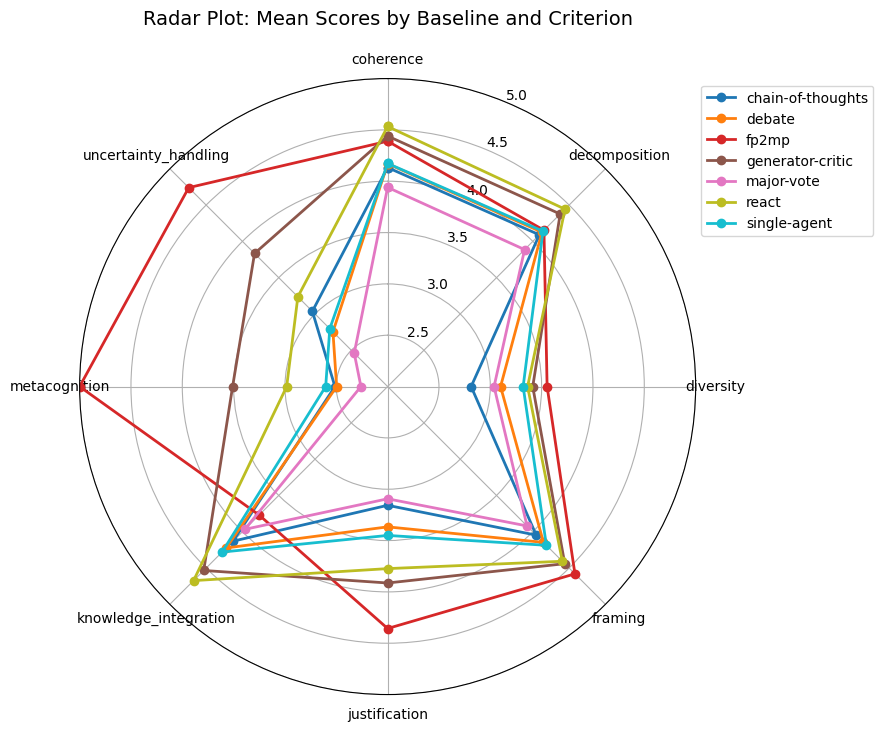
\includegraphics[width=0.85\linewidth]{Sections//5_results//Figures/evaluation_results.png}
    \caption{Radar chart of multi-dimensional evaluation scores across baselines. FP2MP demonstrates stronger performance on reflective reasoning dimensions, particularly metacognition and uncertainty handling.}
    \label{figure:evaluation_results}
\end{figure}

\highlight{To assess whether the observed differences} between FP2MP and the baseline methods are statistically significant, we perform pairwise Wilcoxon signed-rank tests over the 60 paired problem instances for each evaluation criterion.
The resulting $p$-values are reported in Table~\ref{table:p_values}.
The significance threshold is set to $\alpha=0.05$, with underlined values indicating non-significant differences.

\begin{table}[h]
\centering
\small
\resizebox{\textwidth}{!}{
\begin{tabular}{lcccccl}
\hline
\textbf{Criterion} & \textbf{Single Agent}& \textbf{Chain-of-Thought} & \textbf{Actor-Critic} & \textbf{ReAct} 
& \textbf{Majority Voting} 
&\textbf{Debate}
\\
\hline
Coherence & < 0.001& < 0.001& \underline{0.3556}& 0.0194& < 0.001&0.0032\\
Decomposition & \underline{0.7893}& \underline{0.0928}& < 0.001& < 0.001& 0.0011&\underline{0.9103}\\
Diversity & 0.0041& < 0.001& 0.0353& 0.0266& < 0.001&< 0.001\\
Framing & < 0.001& < 0.001& 0.0081& 0.002& < 0.001&< 0.001\\
Justification & < 0.001& < 0.001& < 0.001& < 0.001& < 0.001&< 0.001\\
Knowledge Integration & < 0.001& < 0.001& < 0.001& < 0.001& < 0.001&< 0.001\\
Metacognition & < 0.001& < 0.001& < 0.001& < 0.001& < 0.001&< 0.001\\
Uncertainty Handling & < 0.001& < 0.001& < 0.001& < 0.001& < 0.001&< 0.001\\
\hline
\end{tabular}
}
\caption{
\highlight{Pairwise Wilcoxon signed-rank test} p-values comparing FP2MP with baseline methods across evaluation criteria.
Underlined values indicate comparisons that are not statistically significant ($p \ge 0.05$).
}
\label{table:p_values}
\end{table}

\highlight{Statistical significance is complemented by effect size} analysis using the rank-biserial correlation.
Table~\ref{table:rank_biserial} reports the rank-biserial effect size for each pairwise comparison.
Positive values indicate that FP2MP tends to receive higher scores than the corresponding baseline, while negative values indicate the opposite.
The magnitude of the coefficient reflects the strength of the observed difference, with values close to 1 or $-1$ indicating a strong systematic difference between the paired scores.

\begin{table}[h]
\centering
\small
\resizebox{\textwidth}{!}{
\begin{tabular}{lcccccl}
\hline
\textbf{Criterion} & \textbf{Single Agent}& \textbf{Chain-of-Thought} & \textbf{Actor-Critic} & \textbf{ReAct} 
& \textbf{Majority Voting} 
&\textbf{Debate}
\\
\hline
Coherence & 0.583& 0.671& -0.154& -0.386& 0.788&0.486\\
Decomposition & 0.045& 0.288& -0.724& -0.737& 0.559&0.019\\
Diversity & 0.439& 0.934& 0.338& 0.355& 0.665&0.666\\
Framing & 0.868& 0.979& 0.433& 0.521& 0.946&0.863\\
Justification & 0.992& 0.998& 0.865& 0.936& 1.000&1.000\\
Knowledge Integration & -0.944& -0.824& -1.000& -1.000& -0.470&-0.792\\
Metacognition & 1.000& 1.000& 1.000& 1.000& 1.000&1.000\\
Uncertainty Handling & 1.000& 1.000& 1.000& 1.000& 1.000&1.000\\
\hline
\end{tabular}
}
\caption{
\highlight{Rank-biserial effect sizes} for pairwise comparisons between FP2MP and baseline methods across evaluation criteria.
Positive values indicate higher scores for FP2MP, while negative values indicate higher scores for the corresponding baseline.
}
\label{table:rank_biserial}
\end{table}

\highlight{The statistical results} largely confirm the patterns observed in the mean scores.
FP2MP significantly outperforms all baselines in framing, justification, metacognition, and uncertainty handling, with large positive rank-biserial effect sizes across these dimensions.
In particular, the rank-biserial coefficients for justification, metacognition, and uncertainty handling are consistently close to 1, indicating a systematic advantage of FP2MP rather than a difference driven solely by mean scores.

\highlight{For the remaining dimensions}, the results are more mixed.
FP2MP significantly outperforms Single-Agent, Chain-of-Thought, Majority Voting, and Debate in coherence, while the difference with Actor-Critic is not statistically significant and ReAct performs significantly better.
For decomposition, FP2MP significantly outperforms Majority Voting but does not differ significantly from Single-Agent, Chain-of-Thought, or Debate, while Actor-Critic and ReAct achieve significantly higher scores.
The largest weakness is observed in knowledge integration.
FP2MP is significantly outperformed by every baseline, with particularly large negative rank-biserial effects for ReAct and Actor-Critic.
In contrast, FP2MP significantly outperforms all baselines in diversity, despite diversity not being among the dimensions with the highest absolute scores.

\highlight{Therefore}, FP2MP's main advantage lies in reflective and uncertainty-aware reasoning.
While it shows strong and consistent gains in framing, justification, metacognition, uncertainty handling, and diversity, knowledge integration remains its main weakness.